%% Cubic Ternary Complex Model
%% FigS1CubicTernaryComplexModel.tex
%% Unused packages and definitions removed; TikZ/PGFPlots source formatted.

\documentclass[tikz,margin=2mm]{standalone}

\usetikzlibrary{arrows}

\def\KA{K_A}
\def\KG{K_G}
\def\KL{K_L}

\def\RI{{\rm R}_i}
\def\LRI{{\rm L}{\rm R}_i}
\def\RIG{{\rm R_i}{\rm G}}
\def\LRIG{{\rm L}{\rm R_i}{\rm G}}

\def\RA{{\rm R}_a}
\def\LRA{{\rm L}{\rm R}_a}
\def\RAG{{\rm R_a}{\rm G}}
\def\LRAG{{\rm L}{\rm R_a}{\rm G}}

\def\e{\mathsf{e}}

\begin{document}

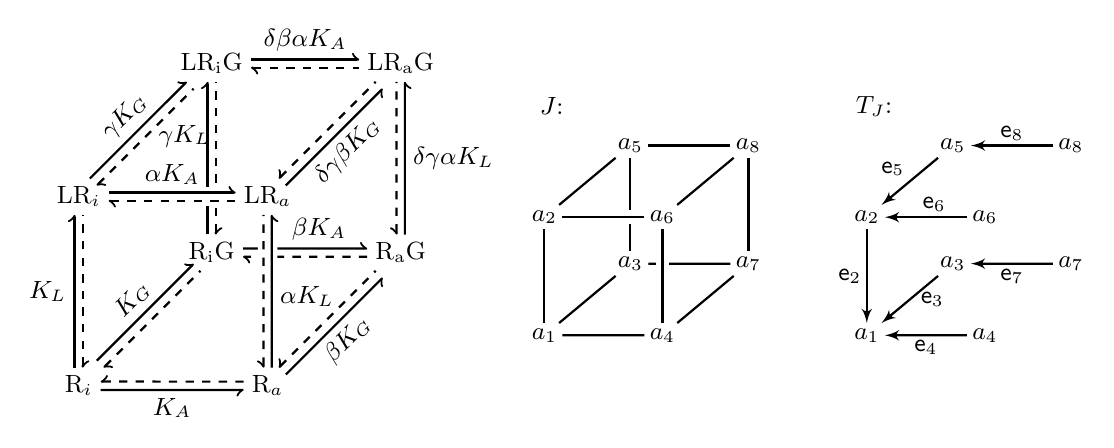
\begin{tikzpicture}[scale=1.3,node distance=1.7cm,>=latex',font=\small,inner sep=2pt,outer sep=1pt]
    \begin{scope}[node distance=2.4cm,yshift=-0.5cm,xshift=0cm]

        \begin{scope}[xshift=1.3cm,yshift=1.3cm]
            \node (LRIG) {$\LRIG$};
            \node[below of=LRIG] (RIG) {$\RIG$};
            \draw[left to-,thick,transform canvas={xshift=-1.5pt}] (LRIG) to node[left,yshift=8pt,xshift=4pt] {$\gamma \KL$} (RIG);
            \draw[dashed,left to-,thick,transform canvas={xshift=1.5pt}] (RIG) to  (LRIG);
            \node[right of=RIG] (RAG) {$\RAG$};
            \draw[-left to,thick,transform canvas={yshift=1.5pt}] (RIG) to node[above,xshift=5pt] {$\beta \KA$} (RAG);
            \draw[dashed,-left to,thick,transform canvas={yshift=-1.5pt}] (RAG) to (RIG);
            \node[right of=LRIG] (LRAG) {$\LRAG$};
            \draw[dashed,right to-,thick,transform canvas={xshift=-1.5pt}] (RAG) to (LRAG);
            \draw[right to-,thick,transform canvas={xshift=1.5pt}] (LRAG) to node[right] {$\delta \gamma \alpha \KL$} (RAG);
            \draw[dashed,left to-,thick,transform canvas={yshift=-1.5pt}] (LRIG) to (LRAG);
            \draw[left to-,thick,transform canvas={yshift=1.5pt}] (LRAG) to node[above] {$\delta \beta \alpha \KA$}  (LRIG);
        \end{scope}

        \begin{scope}
            \node (LRI) {$\LRI$};
            \node[below of=LRI] (RI) {$\RI$};
            \draw[left to-,thick,transform canvas={xshift=-1.5pt}] (LRI) to node[left] {$\KL$} (RI);
            \draw[dashed,left to-,thick,transform canvas={xshift=1.5pt}] (RI) to  (LRI);
            \node[right of=RI] (RA) {$\RA$};
            \draw[-right to,thick,transform canvas={yshift=-1.5pt}] (RI) to node[below] {$\KA$} (RA);
            \draw[dashed,-right to,thick,transform canvas={yshift=1.5pt}] (RA) to (RI);
            \node[right of=LRI] (LRA) {$\LRA$};

            \draw[white,line width=4pt,transform canvas={xshift=-1.5pt}] (RA) to (LRA);
            \draw[white,line width=4pt,transform canvas={xshift=1.5pt}] (LRA) to (RA);

            \draw[dashed,right to-,thick,transform canvas={xshift=-1.5pt}] (RA) to (LRA);
            \draw[right to-,thick,transform canvas={xshift=1.5pt}] (LRA) to node[right,yshift=-2pt] {$\alpha \KL$} (RA);

            \draw[white,line width=4pt,transform canvas={yshift=-1.5pt}] (LRI) to (LRA);
            \draw[white,line width=4pt,transform canvas={yshift=1.5pt}] (LRA) to  (LRI);

            \draw[dashed,left to-,thick,transform canvas={yshift=-1.5pt}] (LRI) to (LRA);
            \draw[left to-,thick,transform canvas={yshift=1.5pt}] (LRA) to node[above,xshift=0pt] {$\alpha \KA$}  (LRI);

        \end{scope}

        \draw[dashed,left to-,thick,transform canvas={xshift=2.5pt}] (RI) to  (RIG);
        \draw[left to-,thick,transform canvas={yshift=2.5pt}] (RIG) to node[midway,above,sloped] {$\KG$} (RI);

        \draw[dashed,left to-,thick,transform canvas={yshift=-2.5pt}] (LRI) to (LRIG);
        \draw[left to-,thick,transform canvas={xshift=-2.5pt}] (LRIG) to node[midway,above,sloped] {$\gamma \KG$} (LRI);

        \draw[dashed,right to-,thick,transform canvas={xshift=-2.5pt}] (RA) to  (RAG);
        \draw[right to-,thick,transform canvas={yshift=-2.5pt}] (RAG) to node[midway,below,sloped] {$\beta \KG$} (RA);

        \draw[dashed,right to-,thick,transform canvas={xshift=-2.5pt}] (LRA) to (LRAG);
        \draw[right to-,thick,transform canvas={yshift=-2.5pt}] (LRAG) to node[midway,below,sloped] {$\delta \gamma \beta \KG$} (LRA);
        %\draw (LRIG) node[above,xshift=-1.8cm,yshift=-0.3cm] {$J$:};
    \end{scope}

    \begin{scope}[scale=0.7,xshift=6.5cm,yshift=-1cm,node distance=1.5cm,outer sep=1pt,inner sep=1pt,shorten >=0pt,shorten <=0pt]
        \node (A2) {$a_2$};
        \node[below of=A2] (A1) {$a_1$};
        \draw[thick] (A2) to node[left] {} (A1);
        \node[right of=A1] (A4) {$a_4$};
        \draw[thick] (A1) to node[below] {} (A4);
        \node[right of=A2] (A6) {$a_6$};
        \draw[thick] (A6) to node[above,xshift=3pt] {} (A2);
        \begin{scope}[xshift=1.2cm,yshift=1cm]
            \node (A5) {$a_5$};
            \node[below of=A5] (A3) {$a_3$};
            \node[right of=A3] (A7) {$a_7$};
            \node[right of=A5] (A8) {$a_8$};
            \draw[thick] (A2) to node[above left] {} (A5);
        \end{scope}
        \draw[thick] (A1) to  node[right,xshift=2pt] {} (A3);
        \draw[thick] (A3) to  node[below] {} (A7);
        \draw[thick] (A5) to  node[above] {} (A8);
        \node[above of=A5,yshift=-1cm,xshift=-1cm] {$J$:};
        \draw[thick] (A6) -- (A8);
        \draw[thick] (A5) -- (A3);
        \draw[thick] (A6) -- (A4);
        \draw[thick] (A4) -- (A7);
        \draw[thick] (A8) -- (A7);

        \draw[line width=5pt,white] (A2) -- (A6);
        \draw[thick] (A2) -- (A6);

        \draw[line width=5pt,white] (A6) -- (A4);
        \draw[thick] (A6) -- (A4);

    \end{scope}

    \begin{scope}[scale=0.7,xshift=11cm,yshift=-1cm,node distance=1.5cm,outer sep=1pt,inner sep=1pt,shorten >=0pt,shorten <=0pt]
        \node (A2) {$a_2$};
        \node[below of=A2] (A1) {$a_1$};
        \draw[->,thick] (A2) to node[left] {$\e_2$} (A1);
        \node[right of=A1] (A4) {$a_4$};
        \draw[<-,thick] (A1) to node[below] {$\e_4$} (A4);
        \node[right of=A2] (A6) {$a_6$};
        \draw[->,thick] (A6) to node[above,xshift=3pt] {$\e_6$} (A2);
        \begin{scope}[xshift=1.2cm,yshift=1cm]
            \node (A5) {$a_5$};
            \node[below of=A5] (A3) {$a_3$};
            \node[right of=A3] (A7) {$a_7$};
            \node[right of=A5] (A8) {$a_8$};
            \draw[<-,thick] (A2) to node[above left] {$\e_5$} (A5);
        \end{scope}
        \draw[<-,thick] (A1) to  node[right,xshift=2pt] {$\e_3$} (A3);
        \draw[<-,thick] (A3) to  node[below] {$\e_7$} (A7);
        \draw[<-,thick] (A5) to  node[above] {$\e_8$} (A8);
        \node[above of=A5,yshift=-1cm,xshift=-1cm] {$T_J$:};
    \end{scope}

\end{tikzpicture}

\end{document}

